\documentclass{beamer}
\usepackage{array}
\usepackage{graphicx}
\usepackage{german}
%\usepackage{txfonts}

\mode<beamer>{%
\usetheme[hideothersubsections,hidetitle]{Hannover}
}
\title[]{Partielle Differentialgleichungen}
\subtitle{1. Sitzung}
\date[24.~Februar 2016]{24.~Februar 2016}
\author{Prof.~Dr.~Andreas M"uller}
\begin{document}

\begin{frame}
\titlepage
\end{frame}

\begin{frame}
\frametitle{Administratives}
\begin{enumerate}
\item Unterrichtsunterlagen $\to$ Moodle
\item "Ubungsbetrieb $\to$ 2h, Aufgaben im Moodle
\item Pr"ufung:
\begin{itemize}
\item f"ur jeden Teil 4 Aufgaben
\item Hilfsmittel $\to$ $2\times 10\times \text{A4}$, Taschenrechner
\end{itemize}
\item Pr"ufungsvorbereitung
\begin{itemize}
\item Aufgabensammlung
\item Moodle-Forum: Fragen und Antworten
\item Pr"ufungen fr"uherer Jahre
\end{itemize}
\end{enumerate}
\end{frame}

\begin{frame}
\frametitle{Zeitplan}
\begin{center}
\includegraphics{zeitplan-1.pdf}
\end{center}
\[
\text{Wirkungsgrad}
=
\frac{1}{\text{Unterrichtszeit}}
\int_0^{100}\text{Aufnahmef"ahigkeit}(t)\,dt
\]
\end{frame}

\begin{frame}
\frametitle{Zeitplan}
\begin{center}
\includegraphics{zeitplan-2.pdf}
\end{center}
\[
\text{Wirkungsgrad}= 50\%
\]
\end{frame}

\begin{frame}
\frametitle{Zeitplan}
\begin{center}
\includegraphics{zeitplan-3.pdf}
\end{center}
\[
\text{Wirkungsgrad}= \color{red}66.6\%
\]
\end{frame}

\begin{frame}
\frametitle{Einf"uhrungsbeispiel}

{\bf Aufgabe:} Stelle die Bewegungsgleichung
einer schwingenden Saite der L"ange $l$ und der Massedichte $\mu$ auf.

\medskip
\pause
{\bf L"osungsansatz:}
Auslenkung $ u(x,t)$ h"angt von Ort $x\in[0,l]$ und Zeit $t\in[0,\infty)$
ab:
\[
u\colon [0,l]\times [0,\infty)\to \mathbb R
\]
\pause
\medskip
\includegraphics{../../skript/images/saite-2.pdf}
\pause
\medskip

{\bf Randbedingung:}
\[
u(0,0)= u(l,0)=0
\]
\end{frame}

\begin{frame}
\frametitle{Bewegungsgleichung}
\includegraphics{../../skript/images/saite-3.pdf}
\vskip 6truecm

\end{frame}

\begin{frame}
\frametitle{Wellengleichung}
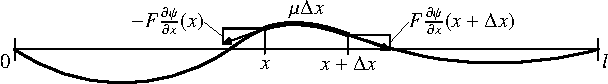
\includegraphics{../../skript/images/saite-1.pdf}
\begin{align*}
\text{Kraft}
=ma
&=
F\frac{\partial u}{\partial x}(x+\Delta x)-F\frac{\partial u}{\partial x}(x)
\\
\\
\mu \Delta x \frac{\partial^2  u}{\partial t^2}
&=
F\frac{\partial u}{\partial x}(x+\Delta x)-F\frac{\partial u}{\partial x}(x)
\\
\\
\frac{\partial^2  u}{\partial t^2}
&=
\frac{F}{\mu}
\frac{\partial^2 u}{\partial x^2},
\qquad
c=\sqrt{\frac{F}{m}}
\end{align*}
Wellengleichung mit Ausbreitungsgeschwindigkeit $c$
\end{frame}

\begin{frame}
\frametitle{H"oheren Dimensionen}
In drei Dimensionen:
\[
\frac{\partial^2 u}{\partial t^2}=c^2
\biggl(
\frac{\partial^2 u}{\partial x^2}
+
\frac{\partial^2 u}{\partial y^2}
+
\frac{\partial^2 u}{\partial z^2}
\biggr)
\]
\pause
Mit Laplace-Operator
\[
\Delta
=
\frac{\partial^2}{\partial x^2}
+
\frac{\partial^2}{\partial y^2}
+
\frac{\partial^2}{\partial z^2}
\]
\pause
einfacher:
\[
\frac{\partial^2 u}{\partial t^2}
=
c^2\Delta  u.
\]
\end{frame}


\begin{frame}
\frametitle{Elektrisches Potential}
Potential 
$\varphi$ 
im Vakuum zwischen den Leitern,
\pause
erf"ullt die partielle Differentialgleichung
\[
\Delta \varphi =0
\]
\pause
{\bf Randbedingung:} Potentiale der Leiter
\end{frame}

\begin{frame}
\frametitle{W"armeleitungsgleichung}
Temperatur $T$ h"angt von Ort und Zeit ab:
\[
T(x,t)
\]
\pause
und erf"ullt die W"armeleitungsgleichung
\[
\frac{\partial T}{\partial t}=\frac{\partial^2T}{\partial x^2}
\]
\end{frame}

\begin{frame}
\frametitle{Was ist eine PDGL}
\begin{enumerate}
\item Was ist eine Differentialgleichung?
\[
\phantom{
F( x_1,\dots,x_n,u,p_1, \dots,p_n) =0,\quad p_i=\frac{\partial u}{\partial x_i}
}
\]
\item Wo ist sie definiert?
\[
\phantom{
\text{Gebiet $\Omega$, d.~h.~offen}
}
\]
\item Randbedingungen?
\[
\phantom{
\text{$u(x)=g(x)$ oder $\frac{\partial u}{\partial n}=g(x)$ auf
$\partial\Omega$}
}
\]
\end{enumerate}
\end{frame}

\begin{frame}
\frametitle{Was ist eine PDGL}
\begin{enumerate}
\item Was ist eine Differentialgleichung?
\[
%\phantom{
F( x_1,\dots,x_n,u,p_1, \dots,p_n) =0,\quad p_i=\frac{\partial u}{\partial x_i}
%}
\]
\item Wo ist sie definiert?
\[
\phantom{
\text{Gebiet $\Omega$, d.~h.~offen}
}
\]
\item Randbedingungen?
\[
\phantom{
\text{$u(x)=g(x)$ oder $\frac{\partial u}{\partial n}=g(x)$ auf
$\partial\Omega$}
}
\]
\end{enumerate}
\end{frame}

\begin{frame}
\frametitle{Was ist eine PDGL}
\begin{enumerate}
\item Was ist eine Differentialgleichung?
\[
%\phantom{
F( x_1,\dots,x_n,u,p_1, \dots,p_n) =0,\quad p_i=\frac{\partial u}{\partial x_i}
%}
\]
\item Wo ist sie definiert?
\[
%\phantom{
\text{Gebiet $\Omega$, d.~h.~offen}
%}
\]
\item Randbedingungen?
\[
\phantom{
\text{$u(x)=g(x)$ oder $\frac{\partial u}{\partial n}=g(x)$ auf
$\partial\Omega$}
}
\]
\end{enumerate}
\end{frame}

\begin{frame}
\frametitle{Was ist eine PDGL}
\begin{enumerate}
\item Was ist eine Differentialgleichung?
\[
%\phantom{
F( x_1,\dots,x_n,u,p_1, \dots,p_n) =0,\quad p_i=\frac{\partial u}{\partial x_i}
%}
\]
\item Wo ist sie definiert?
\[
%\phantom{
\text{Gebiet $\Omega$, d.~h.~offen}
%}
\]
\item Randbedingungen?
\[
%\phantom{
\text{$u(x)=g(x)$ oder $\frac{\partial u}{\partial n}=g(x)$ auf
$\partial\Omega$}
%}
\]
\end{enumerate}
\end{frame}

\begin{frame}
\frametitle{L"osung einer Differentialgleichung}
Differenzierbare Funktion
\[
u\colon \bar\Omega\to\mathbb R
\]
\pause
\begin{enumerate}
\item Differentialgleichung erf"ullt:
\[
F\biggl(x_1,\dots,x_n,u,
\frac{\partial u}{\partial x_1},\dots, \frac{\partial u}{\partial x_n}
\biggr)=0\qquad\text{in $\Omega$}
\]
\pause
\item Randbedingungen erf"ullt
\[
\text{
$u(x)=g(x)$
oder
$\frac{\partial u}{\partial n}(x)=g(x)$
auf
$\partial\Omega$
}
\]
\end{enumerate}
\end{frame}

\begin{frame}
\frametitle{Spezielle Randwertvorgaben}
\begin{enumerate}
\item {\bf Cauchy-Problem:}
\pause
Funktion $u(x,y)$ so, dass die Fl"ache $(x,y,u(x,y))$ eine vorgegebene
Raumkurve enth"alt.
\medskip

\pause
\item {\bf Normalableitung:}
\pause
$n$ Vektor der "ausseren Normalen auf $\partial\Omega$
\[
\frac{\partial u}{\partial n}(x)
=
\frac{d}{dt}u(x+tn)\bigg|_{t=0}
\]
\pause
\item {\bf Gemischte Randwertbedingungen:}
\pause
\[
\underbrace{
\alpha(x) u(x)
}_{\text{Dirichlet}}
+
\underbrace{
\beta(x)\frac{\partial u}{\partial n}
}_{\text{Neumann}}
= g(x) 
\qquad
\text{auf $\partial\Omega$}
\]
\end{enumerate}
\end{frame}

\begin{frame}
\frametitle{Spezialf"alle}
\begin{enumerate}
\item {\bf Lineare PDGL:}

\pause
Funktion
\[
F(x_1,\dots,x_n,u,p_1,\dots,p_n,t_{11},\dots,t_{nn})
\]
ist linear in {\color{red}$u$}, $p_1$,\dots,$p_n$,$t_{11}$,\dots,$t_{nn}$
\pause
\item {\bf Quasilineare PDGL:}

\pause
Funktion
\[
F(x_1,\dots,x_n,u,p_1,\dots,p_n,t_{11},\dots,t_{nn})
\]
ist linear in $p_1$,\dots,$p_n$,$t_{11}$,\dots,$t_{nn}$
\pause
\item {\bf Nichtlineare PDGL}
\end{enumerate}
\end{frame}

\begin{frame}
\frametitle{Ordnungsreduktion}
\[
F\biggl(x,y,u,
\frac{\partial u}{\partial x},
\frac{\partial u}{\partial y},
\frac{\partial^2 u}{\partial x^2},
\frac{\partial^2 u}{\partial x\partial y},
\frac{\partial^2 u}{\partial y^2}
\biggr)=0
\]
\pause
Neue Funktionen:
\[
p(x,y)\qquad\text{und}\qquad q(x,y)
\]
\pause
Neue Gleichungen:
\begin{gather*}
F(x,y,u,p,q,\frac{\partial p}{\partial x},\frac{\partial p}{\partial y},
\frac{\partial q}{\partial y})=0
\\
p=\frac{\partial u}{\partial x}\qquad\text{und}\qquad
q=\frac{\partial u}{\partial y}
\end{gather*}
\pause
Zus"atzlich:
\[
\frac{\partial p}{\partial y}=\frac{\partial q}{\partial x}
\]
\end{frame}



\end{document}
